\chapter{Virtualization and Containerization}

Virtualization and containerization are widely appreciated techniques for distributing multiple instances of applications on single or multiple physical servers. The primary objective of these technologies is to enhance resource utilization and efficiency, while maintaining isolation between applications. The key challenge for virtualization and containerization is to deploy and manage each instance efficiently and consistently across various environments.

\section{Introduction}

One of the major differences between a server cluster and a PC is that the former is usually shared among multiple users or applications at the same time. Though working on the same machine, a user would usually want a private working environment not interrupted by other users. In other words, a user would want to ``virtually'' work on an independent machine with his own CPU, RAM, I/O, OS, drivers and hard disk storage, despite that the actual hardware is shared with others. This can be achieved through \textit{Virtualization}, which enables running multiple operating systems on a single physical server in an uninterrupted and logically separated manner. The virtually independent computer of such kind is often called a \textit{virtual machine} (VM).

Deploying a new VM generally consumes a considerably large amount of time. This is because different VMs on the same server are separated at the OS level, with each VM requiring its own OS installation. Consider a scenario where there are hundreds of small applications (microservices), each requiring a similar but separate environment. Launching VMs for all of them is resource-intensive, particularly when these applications could have shared the same OS kernel and operated within their own isolated workspace.

A more efficient approach would be to deploy a single VM and place each application in a ``container'' with its own customized drivers and configurations. A container is similar to a VM in the sense that it provides a degree of isolation from others, but it is typically ``lighter'' than a VM because it doesn't need to virtualize or duplicate the whole OS as VMs do. This makes containers cheaper to launch and manage.

The technique used to deploy and manage containers is known as ``containerization''. Since a container contains all the configuration and requirement information of an application, running a container on different platforms would consistently generate the same expected result. This has made the sharing and rapid deployment of containers remarkably easy and convenient. The similarities and differences of personal PCs, VMs, and container applications are summarized in Fig. \ref{ch:vac:fig:pcvmcontainersructure}.

\begin{figure}
	\centering
	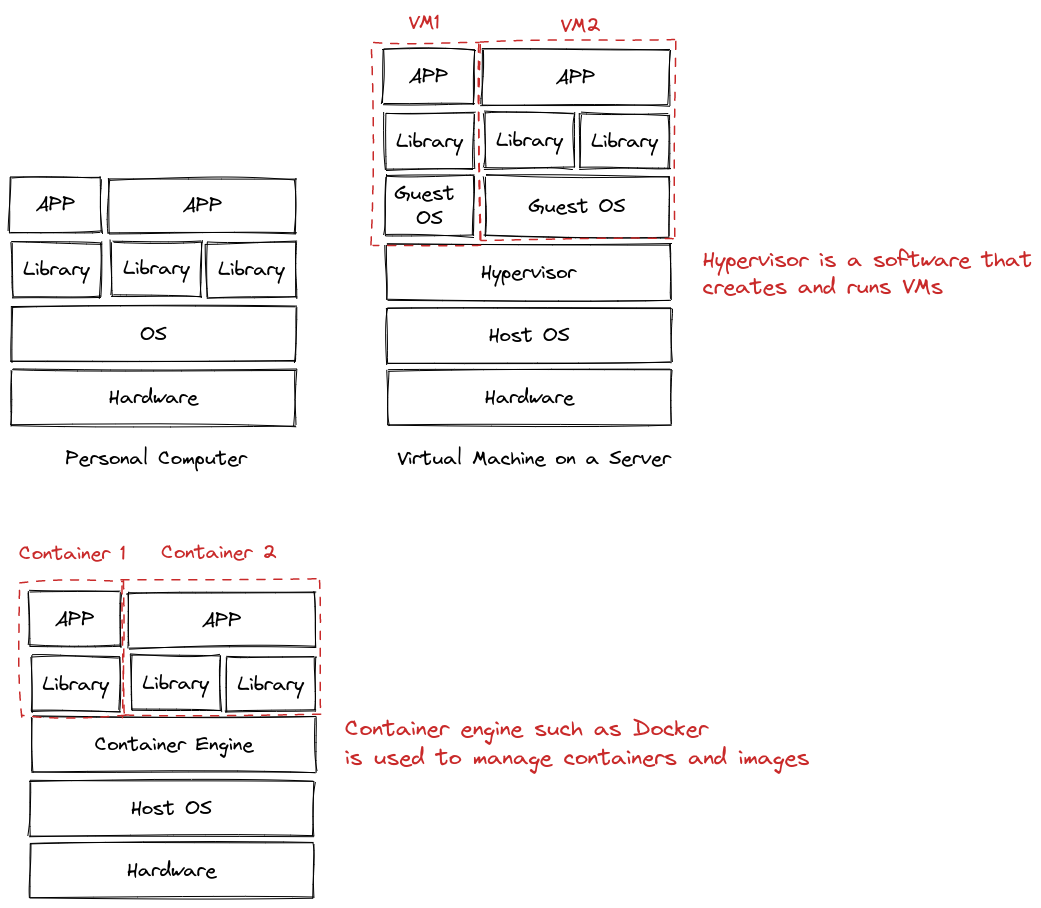
\includegraphics[width=350pt]{chapters/ch-virtualization-and-containerization/figures/pcvmcontainerstructure.png}
	\caption{System architectures of PC, VM and container.} \label{ch:vac:fig:pcvmcontainersructure}
\end{figure}

As an analogy, think of running an APP as asking a kitchen to prepare a dish. The hardware is corresponding with the physical resources in kitchen, such as the cooktop, gas, etc. The OS is corresponding with the person who manages the kitchen, say a cook. The OS needs associated drivers and libraries to run the APP correctly. The drivers and libraries correspond with the skill sets or specific cookers for the dish. Finally, the APP is corresponding with the expected dish.

In the most simple configuration, a dedicated machine is used to run an APP. This is like constructing a dedicated kitchen and hiring a dedicated cook for each dish. The cook is trained to master all necessary skills required for that specific dish. This is shown in Fig. \ref{ch:vac:fig:acookinakitchen}.
\begin{figure}
	\centering
	
\includegraphics[width=300pt]{chapters/ch-virtualization-and-containerization/figures/acookinakitchen.png}
	\caption{PC implementation: a cook in a kitchen.} \label{ch:vac:fig:acookinakitchen}
\end{figure}

In a VM implementation, a larger and more capable kitchen is setup in advance as shown in Fig. \ref{ch:vac:fig:manycooksinakitchen}. For each dish, a cook is hired. Each cook is trained with the skills necessary for his assigned dish. All cooks share the same kitchen. This implementation is more efficient than Fig. \ref{ch:vac:fig:acookinakitchen}, as there is no need to scale up the kitchen for a new dish. By sharing the resources among the cooks, the kitchen can be utilized more effectively.
\begin{figure}
	\centering 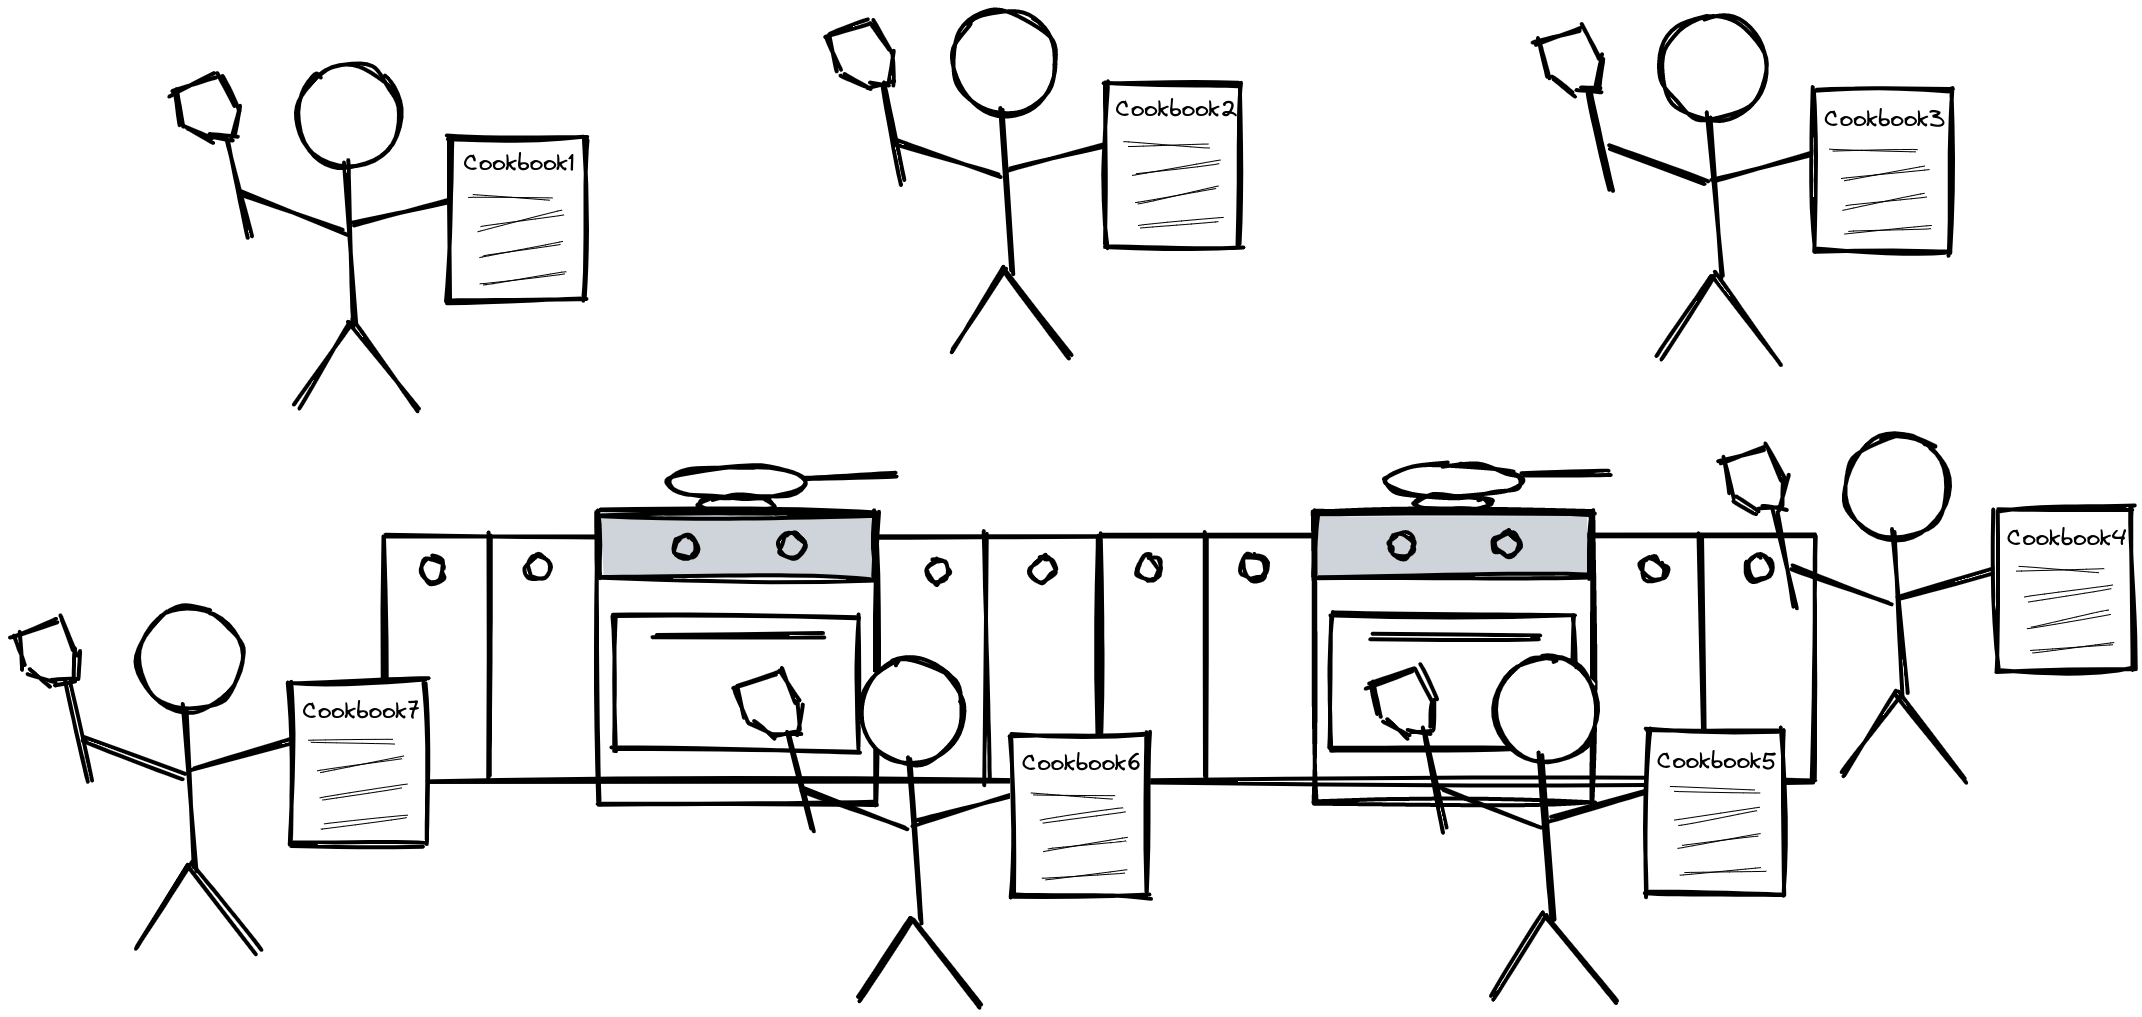
\includegraphics[width=350pt]{chapters/ch-virtualization-and-containerization/figures/manycooksinakitchen.png}
	\caption{VM implementation: many cooks in a kitchen, each with a different cookbook.} \label{ch:vac:fig:manycooksinakitchen}
\end{figure}

While Fig. \ref{ch:vac:fig:manycooksinakitchen} might be a popular practice in many restaurants, it is still too costly to hire a new cook for each dish. In a containerization implementation, a cook usually handles a category of dishes, as shown in Fig. \ref{ch:vac:fig:multitaskcook}. Of course, each dish will stay in its own fry-pan in an isolated way. For each dish, its receipt is provided from where you can find all information required to prepare the dish consistently. As long as the cook is good at multi-tasking, Fig. \ref{ch:vac:fig:multitaskcook} is a more efficient implementation than Fig. \ref{ch:vac:fig:acookinakitchen}.

\begin{figure}
	\centering
	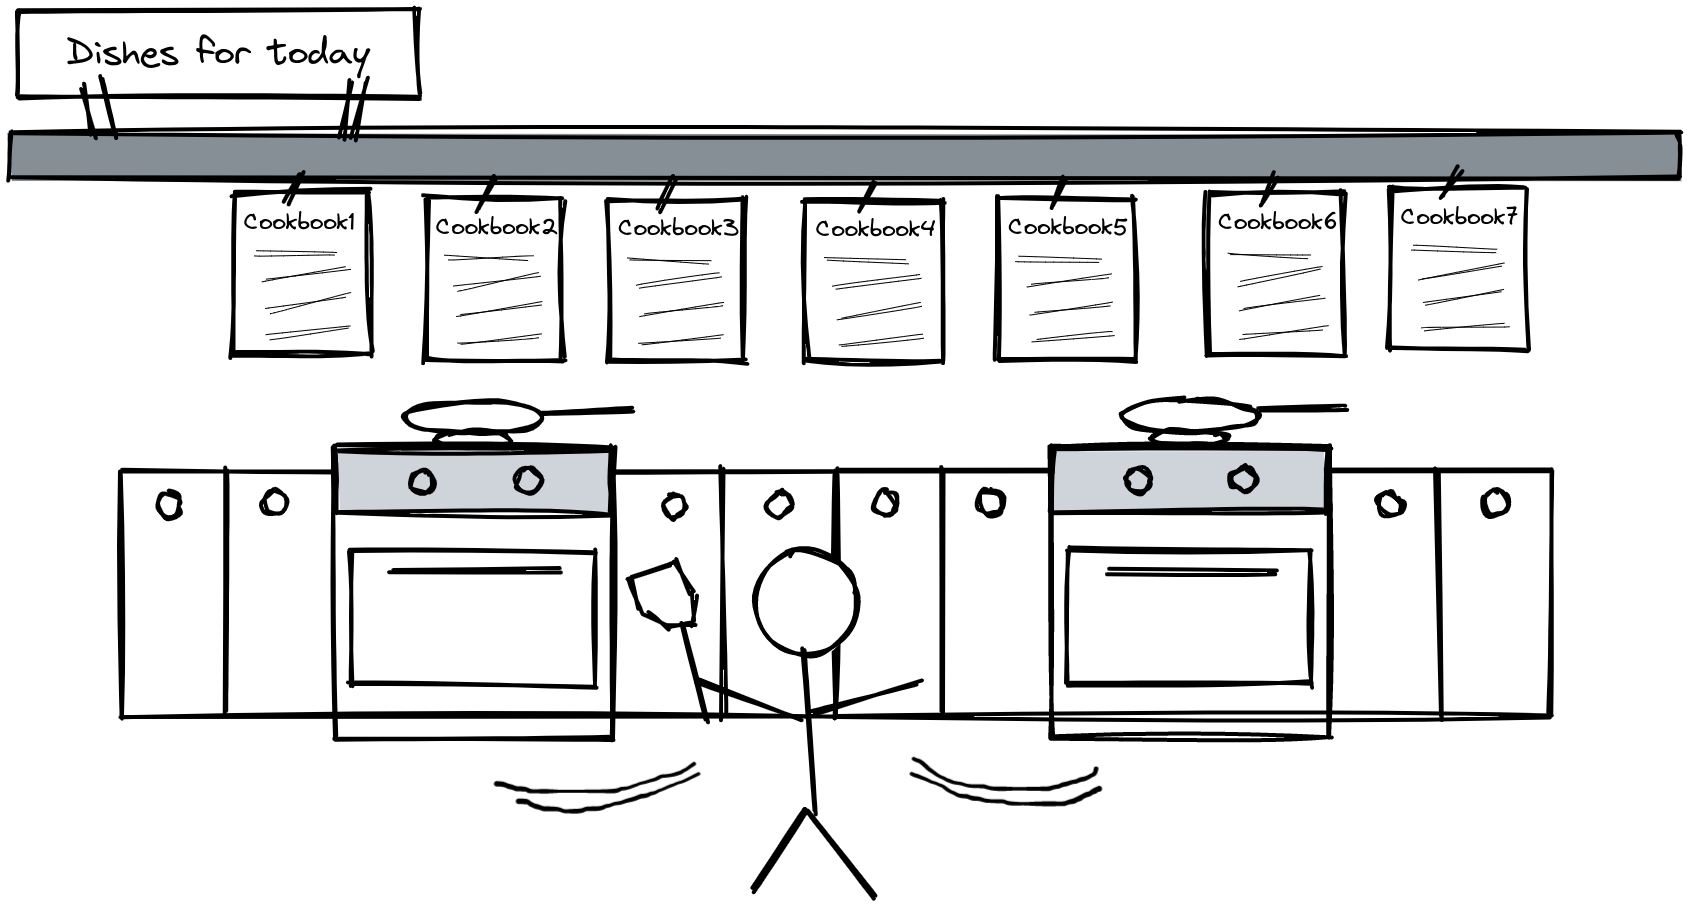
\includegraphics[width=350pt]{chapters/ch-virtualization-and-containerization/figures/multitaskcook.png}
	\caption{Container implementation: one in a kitchen, handling multiple dishes, each has a cookbook and stays in its own pan.} \label{ch:vac:fig:multitaskcook}
\end{figure}

Just like a receipt guaranteeing the consistency of dishes, in containerization, an ``image'' guarantees the consistent performance of container instances. An image is basically a collection of prerequisites and configurations to run a container quickly, efficiently and consistently. Images can be shared among machines to replicate the containers even if the machines adopt different underlying infrastructure such as OS.

\section{Virtualization and Containerization}

Virtualization and containerization technologies have been studied for decades.

Before moving forward to the introduction of containerization approaches, it is important to briefly explain the following frequently used concepts: container runtime, container engine, and container orchestration.

Container runtime refers to the backend software that actually runs the containers. Examples of widely used container runtimes are ``containerd'', ``runc'' and ``cri-o''. Container engine is the interface for a user or software to manage images and containers. Examples of container engines include ``docker'' and ``podman''. Finally, container orchestration is the software that smartly deploy, monitor, restart, and terminate the containers on servers. It is often able to balance API calls, automatically scale up and down the number of running containers, and restart containers upon failure. One of the most widely used container orchestrations is ``kubernetes''.

Container runtime is definitely vital in every containerization implementation. Container engines and container orchestrations must have container runtime built-in. However, the users rarely directly talk to the container runtime. 

Container engine is the interface and management tool of the container runtime, from where the developer can monitor and control the containers manually. Container engines are widely used especially in small projects or in the development environment.

For massive deployment of containers in enterprise-level applications, container orchestration can become handy. In such a case, the container orchestration calls the container engine via API (nowadays a container orchestration may also talk to container runtime directly), instructing it on how the containers should be deployed.

\section{Docker} \label{ch:vac:sec:dc}

This section introduces docker Notice that although docker is famous for docker container engine, docker as a company or community provides many revolutionary container related tools and services that go far beyond a container engine, many of which even used in its opponent container engines.

This section focuses mostly on the introduction of docker engine.

\subsection{Docker Engine VS Alternatives}

Docker engine is the most popular container engines available on the market as of 2023, and it is free of charge for open-source, personal and small business usage. More details of docker can be found at \textit{https://docs.docker.com/}.

But does that mean docker engine is the absolutely best and perfect container engine solution?

Docker has surely revolutionized how we use containerization technology in software development and deployment, and it has been one of the most popular and beloved container engine solutions. However, it is worth mentioning that docker engine is not the only available container engine. For example, as explained earlier podman is an alternative to docker. It supports the same interface (as if podman is an alias) as docker, and claims to have better performance and security. As a matter of fact, RHEL already started the transitionary from docker to podman from RHEL 8. Nowadays, installing docker on the latest versions of RHEL is possible but tedious. On the other hand, install podman (it might be built-in to the OS installation) on RHEL can be done by simply using
\begin{lstlisting}
$ sudo yum install podman
\end{lstlisting}
Kubernetes, a famous container ochestration, is also dropping docker support, as they say ``docker support in the kubelet is now deprecated and will be removed in a future release''. Some may even argue that ``containers are alive, but the role that docker plays is shrinking''. Many open-source initiatives such as podman are gaining round.

Docker has some disadvantages indeed. For one thing, docker uses docker server (docker daemon), a single piece of software running in the backend of the system, to support all the services. This creates a single-point-failure of the system. Docker requires root privileges, and it starts a container on behalf of the root user. This means that the program running inside the container, or the users in the docker group can potentially bypass the OS access control and gain root access, which introduces security risk. These shortages are to some extent addressed by other container engines such as podman which is daemon-less and does not necessarily need to run on root user's behalf.

This is not to say that Docker is falling behind as a whole. Some key techniques that Docker introduced are widely used in all different types and brands of container runtimes and engines. It is just that people do not like some of the features and schematics implementation of Docker engine, and new tools are being developed to fix these problems, the latter of which starting drawing more and more attention. Docker still enjoys widespread usage and support due to its massive community, wealth of online resources, and extensive compatibility with numerous tools and platforms. Nevertheless, for demonstration purpose, for the remaining sections docker is used throughout this notebook. Since podman provides the same interface, it is probable that podman can be used likewise to replicate all the results.

As of 2023, Docker is still the dominating container market engine, with a market share of over $80\%$.

\subsection{Docker Installation}

To install Docker on a Linux machine, go to \textit{https://www.docker.com/} to look for the instruction. The installation steps differ depending on the host machine. As an example, consider installing Docker engine on Ubuntu. Some of the key steps are summarized as follows.

Remove existing Docker engine, if any.
\begin{lstlisting}
$ sudo apt-get remove docker docker-engine docker.io
$ sudo apt-get remove containerd runc
\end{lstlisting}
Add Docker's official GPG key and set up the repository.
\begin{lstlisting}
$ sudo apt-get update
$ sudo apt-get install ca-certificates curl gnupg lsb-release
$ sudo mkdir -p /etc/apt/keyrings
$ curl -fsSL https://download.docker.com/linux/ubuntu/gpg | sudo gpg --dearmor -o /etc/apt/keyrings/docker.gpg
$ echo \
  "deb [arch=$(dpkg --print-architecture) signed-by=/etc/apt/keyrings/docker.gpg] https://download.docker.com/linux/ubuntu \
  $(lsb_release -cs) stable" | sudo tee /etc/apt/sources.list.d/docker.list > /dev/null
\end{lstlisting}
Install Docker.
\begin{lstlisting}
$ sudo apt-get update
$ sudo apt-get install docker-ce docker-ce-cli containerd.io docker-compose-plugin
\end{lstlisting}
To test whether docker is installed correctly, run
\begin{lstlisting}
$ sudo docker run hello-world
\end{lstlisting}
and if everything is done correctly, a message started with ``Hello from Docker!'' will be displayed in the console, together with a brief introduction to how docker works.

Notice that to use docker commands, sudo privilege is required. To avoid typing \verb|sudo| each time running a docker command, add the user to the docker group as follows. In the rest of the section, \verb|sudo| is neglected for docker commands.
\begin{lstlisting}
$ sudo usermod <user name> -aG docker
\end{lstlisting}

Docker installs at least two piece of software on the machine, namely Docker CLI and docker server (also known as docker daemon). The CLI is the interface to the user, and the server is the actual tool that manages images and containers. Docker runs natively on Linux OS. If docker is installed on non-Linux system such as Windows or macOS, ``docker desktop'' is used, which includes a Linux VM to host the docker daemon and run Linux-based containers.

\subsection{Docker Container Management}

To run a container from an image, simply use
\begin{lstlisting}
$ docker run <image>
\end{lstlisting}
Docker will search the local and remote repositories for the image, download the image if necessary, and start a container from that image. By default, after successful execution, the container will enter ``Exited'' status. Use
\begin{lstlisting}
$ docker container ls
\end{lstlisting}
to check the list of running containers, and
\begin{lstlisting}
$ docker container ls -a
\end{lstlisting}
the list of all containers, running or exited. Alternatively, \verb|docker ps|, \verb|docker ps -a| can also be used to list down containers just like \verb|docker container ls|, \verb|docker container ls -a|.

For example, consider running a container of \textit{alpine} as follows. A screen shot is given in Fig. \ref{ch:vac:fig:dockerrunexp}.
\begin{lstlisting}
$ docker run -it --name test-alpine alpine
\end{lstlisting}
where \verb|-i| stands for ``interactive'', which keeps the container's standard input (i.e., the console in this example) open so that the user can actively interact with the container. Option \verb|-t| allocates a pseudo-TTY to the container. TTY stands for ``TeleTYpewriter'', which enforces the I/O of the container following the typical terminal format and allows the user to interact with the container like a traditional terminal, hence making the interactive interface a bit more user-friendly. Finally, \verb|--name| assigns a name to the container. Without an assigned name, docker will assign a random name to the container.
\begin{figure}
	\centering
	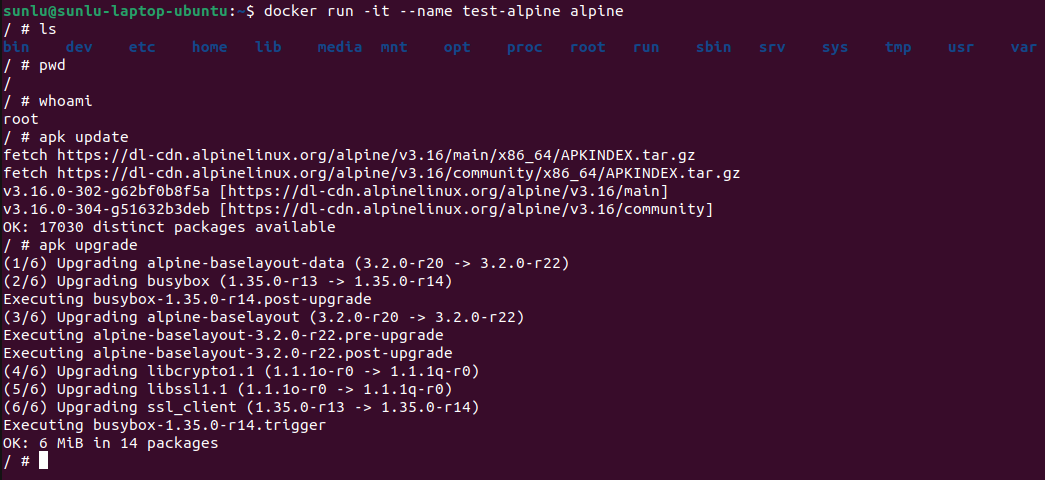
\includegraphics[width=350pt]{chapters/ch-virtualization-and-containerization/figures/dockerrunexp.png}
	\caption{An example of running \textit{apline} container, with interactive TTY and name \textit{test-apline}.} \label{ch:vac:fig:dockerrunexp}
\end{figure}

It can be seen from Fig. \ref{ch:vac:fig:dockerrunexp} that once the container is started, the user can interact with the container via shell, and perform actions such as listing items in the current directory in the container. While keeping the container running, open another terminal and use \verb|docker container ls|. The container \verb|test-alpine| shall appear in the list, as shown in Fig. \ref{ch:vac:fig:dockerrunexppart2}.
\begin{figure}
	\centering
	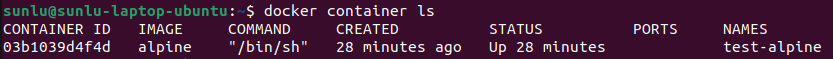
\includegraphics[width=250pt]{chapters/ch-virtualization-and-containerization/figures/dockerrunexppart2.png}
	\caption{List the running container \textit{test-apline}.} \label{ch:vac:fig:dockerrunexppart2}
\end{figure}

After exiting from Fig. \ref{ch:vac:fig:dockerrunexp} (by using \verb|exit| in \textit{alpine}), the container will transfer its status from ``running'' to ``exited'', as shown in Fig. \ref{ch:vac:fig:dockerrunexppart3}.
\begin{figure}
	\centering
	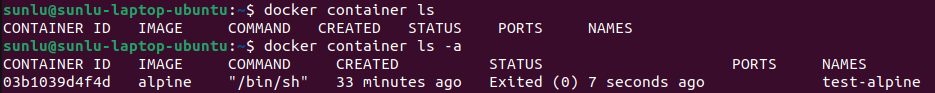
\includegraphics[width=250pt]{chapters/ch-virtualization-and-containerization/figures/dockerrunexppart3.png}
	\caption{List the exited container \textit{test-apline}.} \label{ch:vac:fig:dockerrunexppart3}
\end{figure}

It is also possible to launch a container and let it run in the backend using \verb|-d| flag which stands for ``detached mode''. An example is given below.
\begin{lstlisting}
$ docker run -dt --name test-background-alpine alpine
\end{lstlisting}
By changing \verb|-i| to \verb|-d|, the container runs in the backend silently. The status of the container, after executing the above command, will stay running and can be displayed by \verb|docker container ls|.

Commonly used commands regarding launching a container are given in Tables \ref{ch:vac:tab:launchcontainer}, and \ref{ch:vac:tab:listcontainer}.

\begin{table}
	\centering \caption{Commonly used docker commands to launch a container.}\label{ch:vac:tab:launchcontainer}
	\begin{tabularx}{\textwidth}{llX}
		\hline
		Command & Flag & Description \\ \hline
		\verb|docker run| & --- & Launch a container of the image followed by the command. If the image cannot be found locally, it downloads the image from the remote repository automatically. Assign a random name to the container. Exit the container after execution. \\ \hdashline
        \verb|docker run| & \verb|-i| & Keep the standard input of the container open when launching the container. \\ \hdashline
        \verb|docker run| & \verb|-d| & Launch the container in the backend and keep it running. \\ \hdashline
        \verb|docker run| & \verb|--rm| & Automatically remove the container when exiting. The removed container will not be listed in \verb|docker container ls -a|. This is usually used for testing and debugging. \\ \hdashline
        \verb|docker run| & \verb|-t| & Allocate a pseudo-TTY. The flag usually comes with the flags \verb|-i| or \verb|-d|, to form \verb|-it| or \verb|-dt|. \\ \hdashline
        \verb|docker run| & \verb|--restart| & Enforce restart of the container upon exiting. This is usually used on containers running in the backend. Commonly used restart configurations include \verb|--restart no| (do not restart), \verb|--restart on-failure[:<max retries>]| (restart if exits with an error flag), \verb|--restart always| (always restart when exists). \\ \hdashline
        \verb|docker run| & \verb|--name| & Assign a name to the container. \\
		\hline
	\end{tabularx}
\end{table}

\begin{table}
	\centering \caption{Commonly used docker commands to display local images and containers.}\label{ch:vac:tab:listcontainer}
	\begin{tabularx}{\textwidth}{llX}
		\hline
		Command & Flag & Description \\ \hline
        \verb|docker image ls| & --- & List local images. \\ \hdashline
        \verb|docker container ls| & --- & List running containers. \\ \hdashline
        \verb|docker container ls| & \verb|-a| & List all containers. \\
		\hline
	\end{tabularx}
\end{table}

To re-start an existing but exited container, use
\begin{lstlisting}
$ docker start <container>
\end{lstlisting}
This command starts the exited container, and keep it running in the backend.

For a container running in the backend, use \verb|docker exec| to execute a shell command in that container as follows.
\begin{lstlisting}
$ docker exec <container> <command>
\end{lstlisting}

To enable the TTY shell of a container running in the backend, use
\begin{lstlisting}
$ docker exec -it <container> <shell name>
\end{lstlisting}
Notice that the shell used by the application running inside the container may differ from the one used in the host machine. In the case of an \textit{alpine} image based container, \verb|ash| is the default shell. For a \textit{ubuntu} image based container, \verb|bash| is often used. To exit from the TTY shell while keep the container running in the backend, use shortcut key \verb|Ctrl+p+q|.

An alternative way to interact with containers running in the backend is to use
\begin{lstlisting}
$ docker attach <container>
\end{lstlisting}
to attach local standard input, output, and error streams to a running container. Similar with the previously introduced \texttt{docker exec -it} command, \texttt{docker attach} also starts the shell of the application running in the container. Use \verb|Ctrl-C| to quite the shell.

To check the processes that is running in the container, use
\begin{lstlisting}
$ docker top <container>
\end{lstlisting}

There are multiple ways and protocols to access the files in a container, depending on the I/O setup of the container. For a container running locally, \verb|docker cp| can be used for file transfer between the container and the host machine as follows. From container to host machine:
\begin{lstlisting}
$ docker cp <container>:<source> <destination>
\end{lstlisting}
and from host machine to container:
\begin{lstlisting}
$ docker cp <source> <container>:<destination>
\end{lstlisting}
where \verb|<source>| and \verb|<destination>| refer to the path to the source and destination, respectively, located in the host machine or the container.

To stop, kill (force stop) or restart a container running in the backend, use
\begin{lstlisting}
$ docker stop <container>
$ docker kill <container>
$ docker restart <container>
\end{lstlisting}
respectively. When a container is stopped, it enters exited status. To remove an exited container or all exited containers, use
\begin{lstlisting}
$ docker container rm <container>
\end{lstlisting}
or
\begin{lstlisting}
$ docker container prune
\end{lstlisting}
respectively. To rename a container (without changing its container ID or anything else), use
\begin{lstlisting}
$ docker rename <container-old-name> <container-new-name>
\end{lstlisting}

To quickly check container status including resource consumption (CPU, memory usage, etc.), use
\begin{lstlisting}
$ docker stats [<container>]
\end{lstlisting}
where the user can choose to list down all containers or a specified container. To show more detailed information of a container, including its status, gateway, IP address, etc., use
\begin{lstlisting}
$ docker inspect <container>
\end{lstlisting}
Finally, to check the logs of a container (e.g., its standard output to the console), use
\begin{lstlisting}
$ docker logs <container>
\end{lstlisting}

A container is usually generated from an image. It is also possible to do vise versa, i.e., packaging a container into an image. To create an image from a container, use
\begin{lstlisting}
$ docker commit <container> <image>
\end{lstlisting}
where \verb|docker commit| command saves the container's file changes or settings into a new image, which allows easier populating containers or debugging in a later stage. Notice that \verb|docker commit| does not save everything of the container into the image, and it is not the only way an image is created.

A container can be configured accessible from not only the host machine but also other computers in LAN or the Internet. In a typical web service application, the host machine and the containers are often designed following the architecture similar with Fig. \ref{ch:vac:fig:containerwebserverarchitecture}. Notice that in practice, the load balancer and the containers may or may not run on the same physical machine.

The load balancer is a container orchestration that monitors the status of the containers, manages the data flow, and scales up and down the number of containers depending on the total load. In case where there are multiple physical servers, the load balancer is run on a ``master'' server, and the containers are distributed on multiple ``slave'' servers, each of which is called a ``worker node'', or ``node'' for simplicity. Container engines are installed on each and every node. The load balancer talks with the container engines on each node to deploy containers. The APP instances such as \textit{apache} or \textit{nginx} shall run in the containers distributively.
\begin{figure}
	\centering
	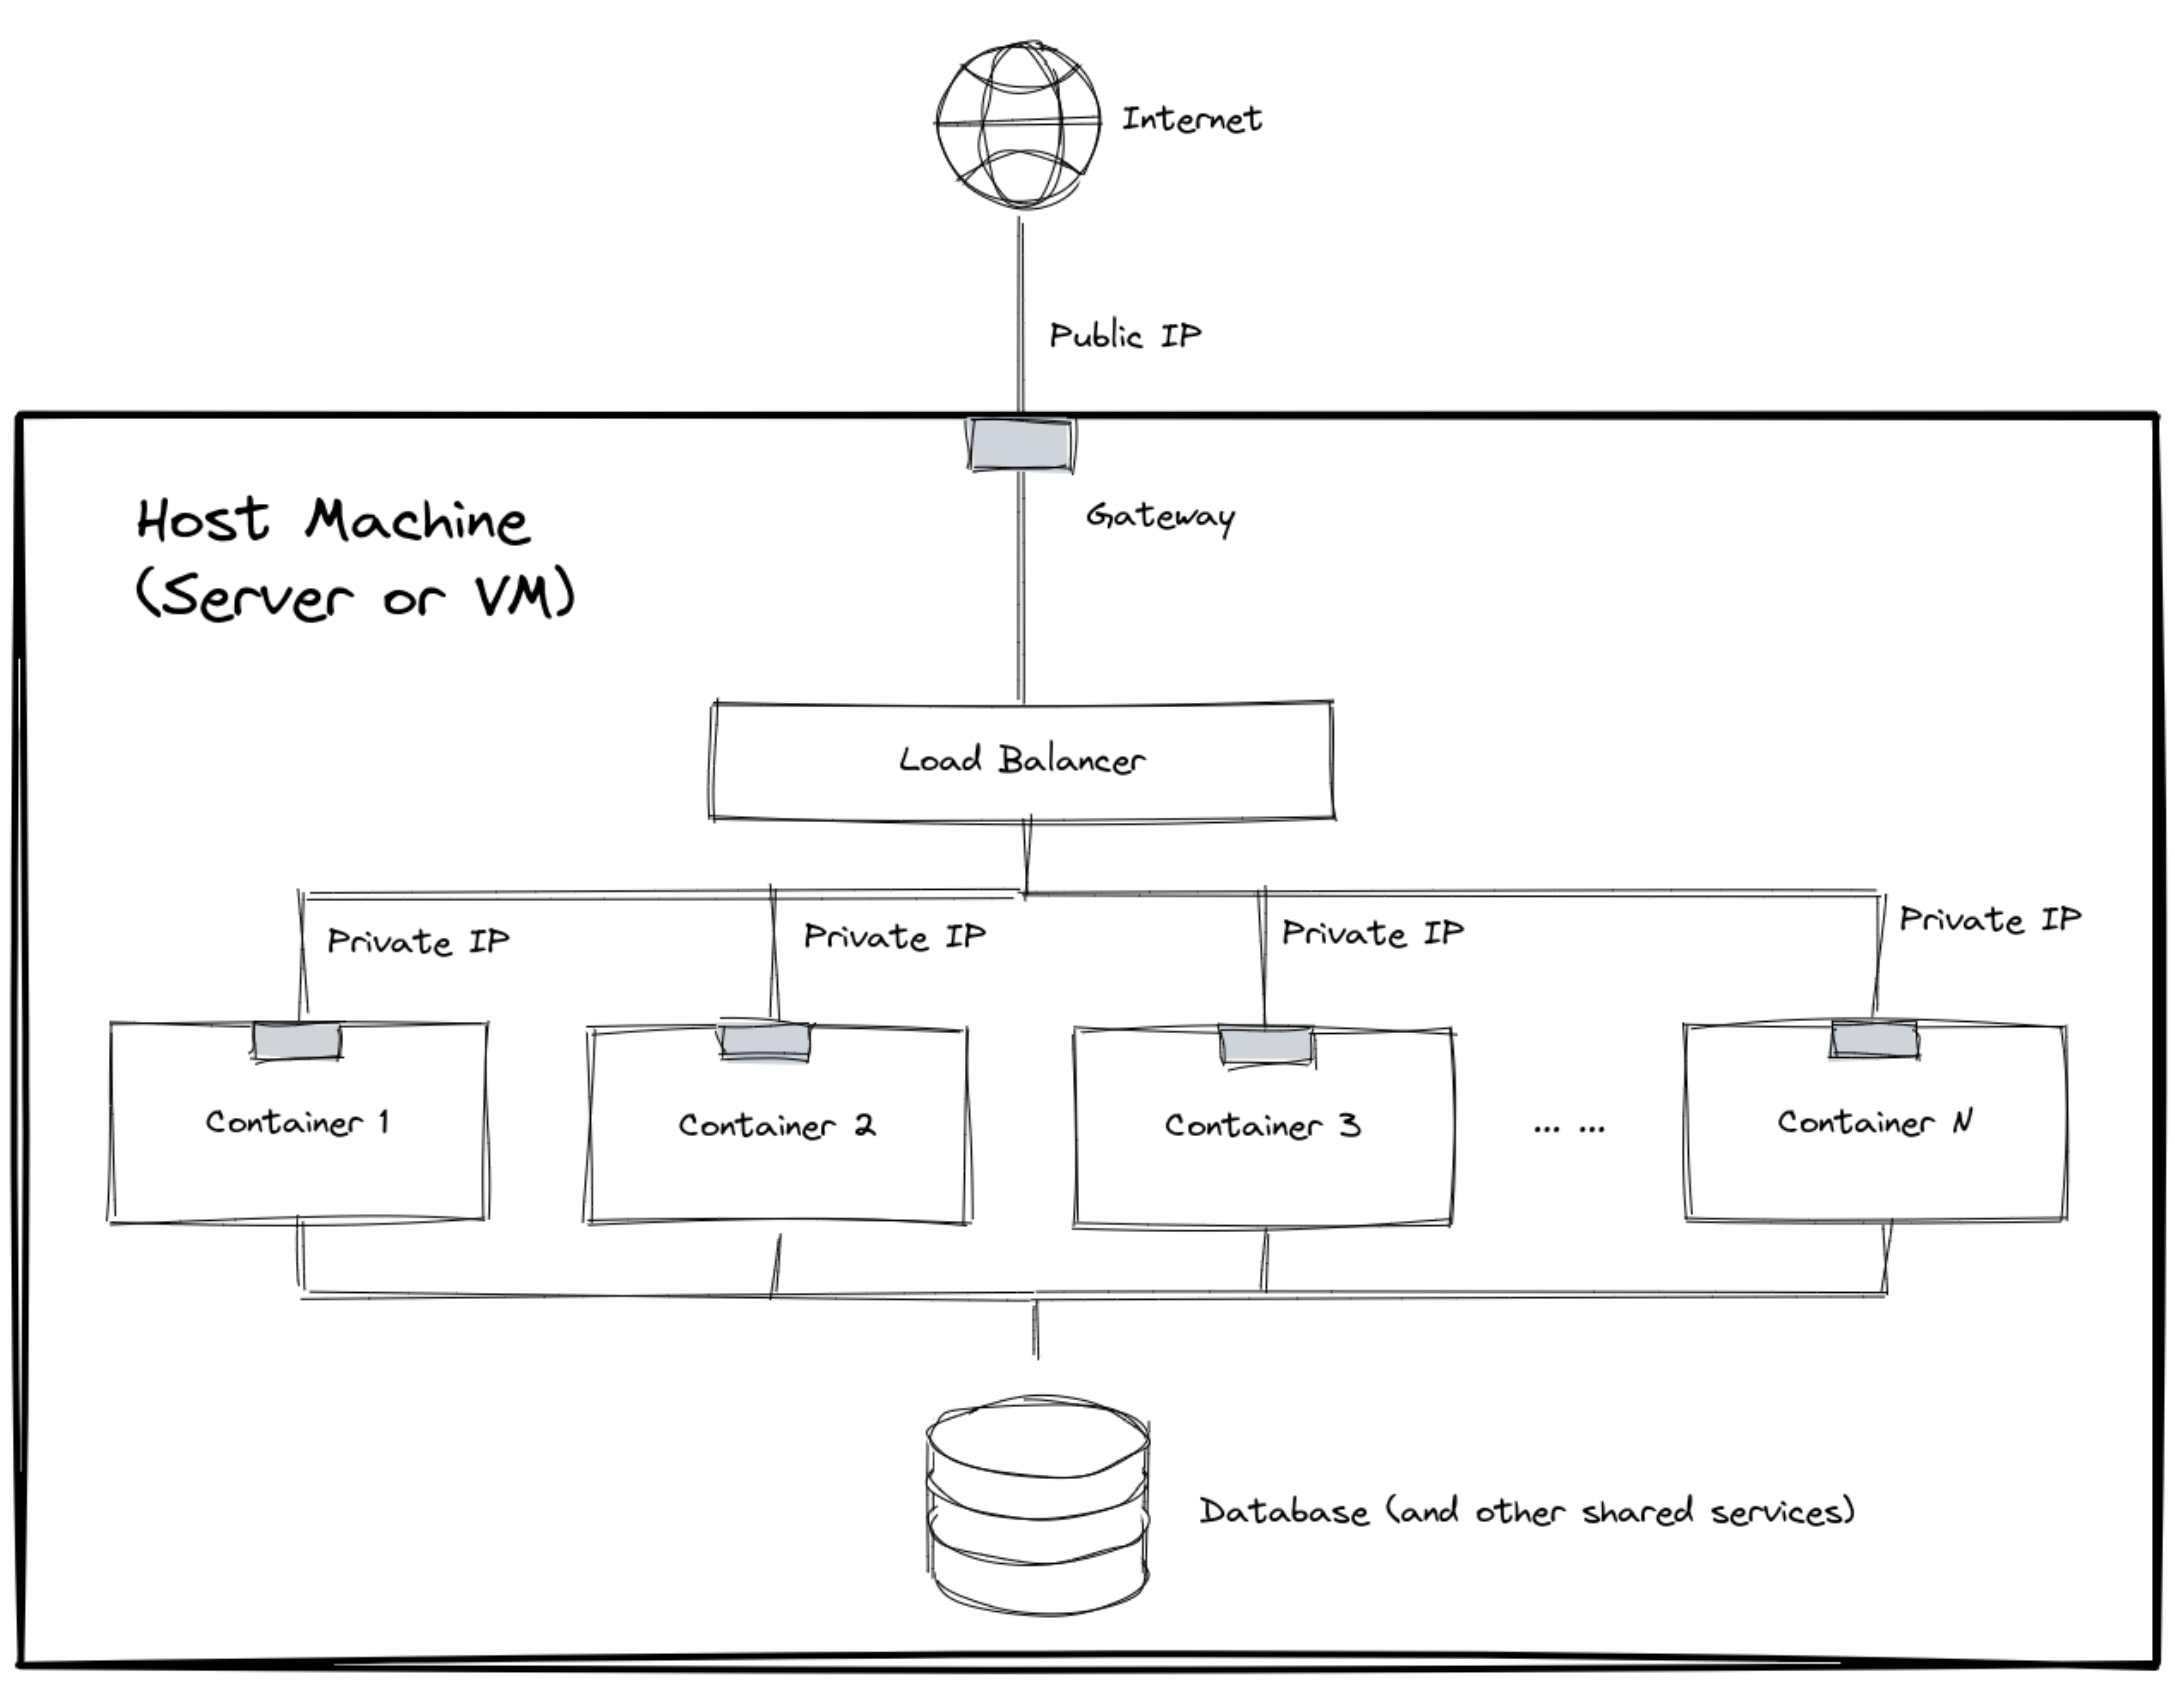
\includegraphics[width=350pt]{chapters/ch-virtualization-and-containerization/figures/containerwebserverarchitecture.png}
	\caption{A simplified architecture where containers are used to host the web service.} \label{ch:vac:fig:containerwebserverarchitecture}
\end{figure}

An example of setting up a web server in containers from scratch is given in this section. For simplicity, everything happens on a single physical server. Only one container is used and the load balancer and the shared services are not included in the example.

As a first step, create a container from the official \textit{nginx} image as follows. Notice that it is also possible to create a container from \textit{apline}, and install \textit{nginx} on \textit{apline}.
\begin{lstlisting}
$ docker run -dt --name simple-web nginx
\end{lstlisting}

Next, create the configuration file for \textit{nginx}, and also the \textit{html} files to be used as the static web page. For convenience, the files are created and edited in the host machine, then copied to the container. The following \textit{default.conf} and \textit{index.html} have been created, respectively. The configuration file \textit{default.conf} is given below.
\begin{lstlisting}
server {
	listen 80 default_server;
	listen [::]:80 default_server;
	root /var/www/html/;
}
\end{lstlisting}
The \textit{html} file \textit{index.html} is given below.
\begin{lstlisting}
<html>
	<body>
		<h1>Hello World!</h1>
	</body>
</html>
\end{lstlisting}
Use \verb|docker copy| to copy the two files to the designed locations in the container as follows.
\begin{lstlisting}
$ docker exec simple-web mkdir -p /var/www/html
$ docker cp default.conf simple-web:/etc/nginx/conf.d/default.conf
$ docker cp index.html simple-web:/var/www/html/index.html
\end{lstlisting}
where \verb|mkdir -p| creates the directories along the given path, if not exist. Notice that the file name in the destination can be ignored if it is the same with the source, i.e., the copy commands can be replaced by
\begin{lstlisting}
	$ docker cp default.conf simple-web:/etc/nginx/conf.d/
	$ docker cp index.html simple-web:/var/www/html/
\end{lstlisting}

Change the ownership of the \textit{html} file as follows, so that the current user \textit{nginx} is able to access that file.
\begin{lstlisting}
$ docker exec simple-web chown -R nginx:nginx /var/www/html
\end{lstlisting}

Finally, reload and configuration file and restart the web server as follows.
\begin{lstlisting}
$ docker exec simple-web nginx -s reload
\end{lstlisting}

To test the web server running inside the container, obtain the IP address of the container using
\begin{lstlisting}
$ docker inspect simple-web | grep IPAddress
\end{lstlisting}
and open a browser to key in the obtained IP address. If everything is done correctly, the browser should try to access port 80 of the container, and the ``Hello World!'' web page shall show up.

For easy sharing and populating of the container, commit the container into a new image using \verb|docker commit| as follows. The new image can be used to populate the web server, just like ``web01'' container given below.
\begin{lstlisting}
$ docker commit simple-web simple-web-image
$ docker run -dt --name web01 -p 80:80 simple-web-image
\end{lstlisting}
where \verb|-p <host machine port>:<container port>| is used to map ports. Notice that different from the previous container ``\textit{simple-web}'', the new container ``\textit{web01}'' IP address port 80 is mapped with the port 80 of the host machine. Therefore, the web page hosted in ``\textit{web01}'' can be accessed not only by the host machine, but also by other machines in the same network with the host machine.

\subsection{Docker Volume Configuration} \label{ch:vac:subsec:dockervolume}

As introduced earlier, \verb|docker cp| can be used to transfer data into and out of a container. An alternative way of accessing docker container data from the host machine is to use docker volume. Docker volume is used to mount host machine hard drive to container storage. Details are introduced below.

To create a docker volume, use
\begin{lstlisting}
$ docker volume create <volume>
\end{lstlisting}
To list down volumes and to inspect a volume, use
\begin{lstlisting}
$ docker volume ls
$ docker volume inspect <volume>
\end{lstlisting}
respectively. Finally to remove a volume or all volumes, use
\begin{lstlisting}
$ docker volume rm <volume>
$ docker volume prune
\end{lstlisting}
respectively.

When starting a container from an image, volumes can be mapped with the internal storage inside the container by using
\begin{lstlisting}
$ docker run -v <volume>:<container-internal-path>[:ro] <image>
\end{lstlisting}
which should synchronize \verb|<volumn name>| with \verb|<container internal path>|. The optional \verb|:ro| can be specified if it is a read-only volume. Instead of using a volume name, the path to a directory in the host machine can also be used, in which case the specified directories in the host machine and in the container should be synchronized.

Docker volume guarantees data persistence in containerized applications. When a docker container is removed, any data written to the container's writable layer is lost. Docker volumes, however, are stored outside of the container's writable layer, allowing data to persist even after the container is removed. This persistence is particularly important for applications that require permanent storage, such as databases.

Moreover, Docker volumes can be shared among multiple containers, which facilitates data exchange and allows containers to work on the same dataset. Therefore, Docker volumes are not just a tool for data persistence, but also an effective mechanism for data sharing and collaboration among containers.

The data persists in the Docker host, and from the container's perspective, it is treated as a mounted volume. Hence, the data is not duplicated physically.


\subsection{Docker Image Management} \label{ch:vac:sec:di}

In earlier Section \ref{ch:vac:sec:dc}, images were used to create containers. An image performs like a blueprint that encapsulates all the necessary information needed to spawn a container. It includes initial configurations, requisite libraries, and other pertinent metadata. Docker images are highly portable and can be shared across various machines and platforms. This section delves deeper into the construction and functionality of Docker images.

An image shall contain everything needed to create and initialize a container. This include but not limited to:
\begin{itemize}
  \item Necessary steps (also known as ``layers'') to create a container.
  \item Application code that is to run in the containers
  \item Files to support the application
  \item Libraries, tools and dependencies
\end{itemize}
In addition, an image shall be designed and organized in such a way that it is migratable, reusable and light, and can be used to easily populate large number of containers. For better inheritability, an image might be based on another existing image, which is called its parent image. An image with no parent, such as the official \textit{hello-world} image from Docker Hub, is called a base image.

The Dockerfile is a text document that serves as the blueprint for constructing a Docker image, as illustrated in Fig. \ref{ch:vac:fig:dockerfiletoimage}. Notably, the Dockerfile itself isn't included within the resulting image.

\begin{figure}
	\centering
	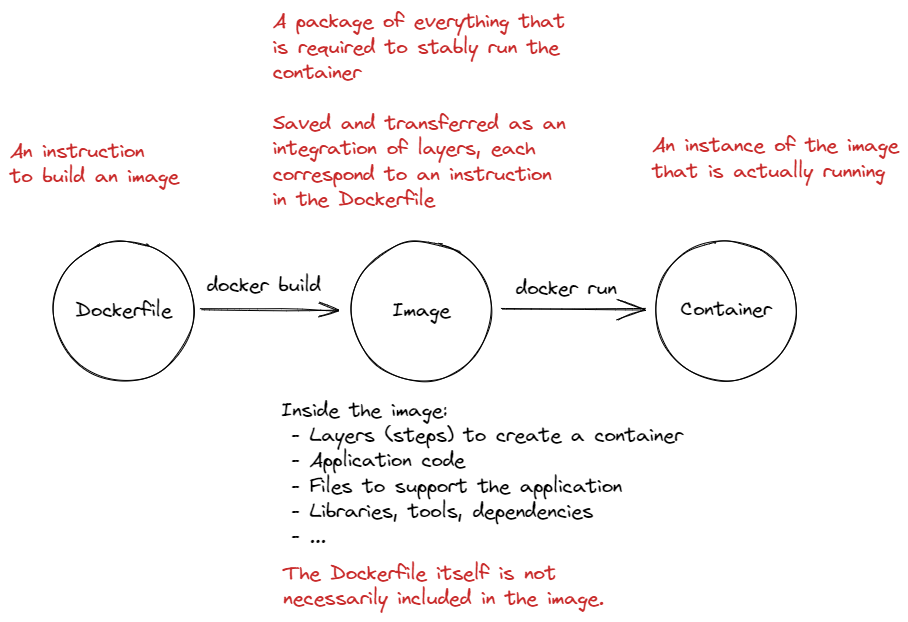
\includegraphics[width=350pt]{chapters/ch-virtualization-and-containerization/figures/dockerfiletoimage.png}
	\caption{A demonstration of how Dockerfile, image and container link to each other.} \label{ch:vac:fig:dockerfiletoimage}
\end{figure}

Since a Docker image's primary role is to serve as a template for containers, many Dockerfile commands appear like a ``step-by-step'' recipe for container creation. Each instruction corresponds to an ``image layer''. An image is, in essence, an amalgamation of these layers. It is stored and distributed in this format. If images share layers (for instance, different versions of the same app), these shared layers aren't saved or transferred redundantly, resulting in significantly reduced image sizes. More details can be found at \textit{https://docs.docker.com/storage/storagedriver/}.

Docker containers employ a special file system known as the Union File System (UFS), which is well suited to the ``layer'' concept. UFS facilitates file sharing between the container and the host machine, along with combining read-only upper layers and writable lower layers, among other functions. A demonstration to illustrate this concept is given later in Fig. \ref{ch:vac:fig:dockerlayerdemo}.

Just as a quick example, the Dockerfile to build the official \textit{hello-world} image from Docker Hub looks like the following.
\begin{lstlisting}
FROM scratch
COPY hello /
CMD ["/hello"]
\end{lstlisting}
Like other computer languages, Dockerfiles have reserved keywords, environment variables, and syntax rules. Only the basics of constructing a Dockerfile are introduced in this section. More details can be found in the Docker reference on the official website. In the example above, \verb|FROM scratch| signifies that this image is a base image without a parent. The \verb|COPY hello /| instruction copies the \textit{hello} binary script from the image to the root directory of the container. Lastly, \verb|CMD ["/hello"]| runs the \textit{hello} binary script.

In general, a typical Dockerfile includes the following instructions to build an image. These instructions allow the image to know how to create a container, automatically construct the file system directory structure, install necessary packages, and run the app:
\begin{enumerate}[(1)]
  \item Define parent image.
  \item Create filesystem directory.
  \item Set working directory.
  \item Copy files.
  \item Configure registry.
  \item Install packages.
  \item Copy more files after package installation.
  \item Switch to the correct user.
  \item Expose port.
  \item Run the APP.
\end{enumerate}

The keywords to be used in a Dockerfile to realize the above instructions, such as \verb|FROM|, \verb|RUN|, and many more, are explained in Table \ref{ch:vac:tab:keywordsdockerfile}.

\begin{table}
	\centering \caption{Critical keywords used in a Dockerfile.}\label{ch:vac:tab:keywordsdockerfile}
	\begin{tabularx}{\textwidth}{lX}
		\hline
		Syntax & Description \\ \hline
		\verb|FROM <image>| & Define the parent image. A Dockerfile must start with a \verb|FROM| instruction. A Dockerfile can contain multiple \verb|FROM| instructions, in which case the last \verb|FROM| statement is the final base image and the earlier \verb|FROM| instructions creates intermediate images that can be used in the final image. An optional \verb|:<tag>| following \verb|<image>| can be used to specify the version of the image to use as the base. By default, the latest version of the image is used. \\ \hdashline
		\verb|RUN <command>| & Execute a shell command using \verb|/bin/sh -c|. \\ \hdashline
		\verb|WORKDIR <path>| & Set the working directory from the point onward. This prepares the working directory for the upcoming \verb|RUN|, \verb|COPY|, etc., commands. \\ \hdashline
		\verb|ADD <src> <dest>| & Add (Copy) \verb|<src>|, either a directory/file or URL, to \verb|<dest>|. An optional \verb|[--chown=<user>:<group>]| can be used to specify the owner and group of the added files. \\ \hdashline
		\verb|COPY <src> <dest>| & Copy \verb|<src>|, a directory/file, to \verb|<dest>|. An optional \verb|[--chown=<user>:<group>]| can be used to specify the owner and group of the added files. Notice that \verb|COPY| is similar with \verb|ADD|. \verb|COPY| is easier but less powerful than \verb|ADD|. It cannot handle tar or URL. \\ \hdashline
		\verb|USER <user>| & Switch user for the instructions beyond this point. \\ \hdashline
		\verb|EXPOSE <port>| & Specifies the ports that the container shall listen to. An optional \verb|/<protocol>| following \verb|<port>| can be used to specify the protocol for communication. \\ \hdashline
		\verb|CMD ["<exe>", "p1", ...]| & As the last instruction of a Dockerfile, run the APP. Notice that a Dockerfile can only contain one \verb|CMD| instruction. The executable command name and the parameters are put into a list. \\
		\hline
	\end{tabularx}
\end{table}

Besides Table \ref{ch:vac:tab:keywordsdockerfile}, there are other Dockerfile keywords that can significantly simplify the design and maintenance of the image. For example, \verb|ENV <key>=<value>| assign a value to an environmental variable; \verb|LABEL <key>="<value>"| assigns a tag to the image, which can be displayed when \verb|docker inspect <container>| is used.

Examples of Dockerfiles are given below, one from \textit{docs.docker.com} and the other from Linux Academy.

The docker image layer structure of the second example is given in Fig. \ref{ch:vac:fig:dockerlayerdemo} as a demonstration. Notice that in Fig. \ref{ch:vac:fig:dockerlayerdemo}, \verb|bootfs| refers to the ``boot file system'', including the bootloader and the Linux kernel. Upon run, a container layer will be added to the image, as shown by the blue dashed box in Fig. \ref{ch:vac:fig:dockerlayerdemo}. In the container, all the changes made is saved into the container layer.

To generate a new image to include the changes made in the container, use \verb|docker commit|, which essentially commits the container layer as the latest image layer in the new image, as shown by the green dashed box in Fig. \ref{ch:vac:fig:dockerlayerdemo}.

\begin{lstlisting}
# First Example
FROM golang:1.16
WORKDIR /go/src/github.com/alexellis/href-counter/
RUN go get -d -v golang.org/x/net/html
COPY app.go ./
RUN CGO_ENABLED=0 GOOS=linux go build -a -installsuffix cgo -o app .

FROM alpine:latest
RUN apk --no-cache add ca-certificates
WORKDIR /root/
COPY --from=0 /go/src/github.com/alexellis/href-counter/app ./
CMD ["./app"]
\end{lstlisting}

\begin{lstlisting}
# Second Example
FROM node:10-alpine
RUN mkdir -p /home/node/app/node_modules && chown -R node:node /home/node/app
WORKDIR /home/node/app
COPY package*.json ./
RUN npm config set registry http://registry.npmjs.org/
RUN npm install
COPY --chown=node:node . .
USER node
EXPOSE 8080
CMD ["node", "index.js"]
\end{lstlisting}

\begin{figure}
	\centering
	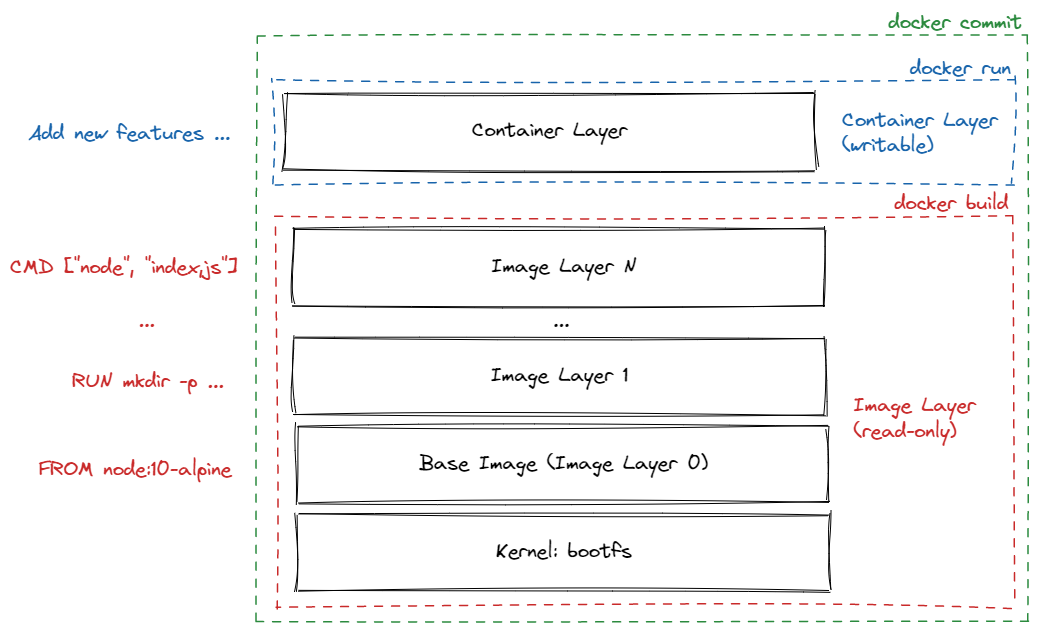
\includegraphics[width=350pt]{chapters/ch-virtualization-and-containerization/figures/dockerlayerdemo.png}
	\caption{A demonstration of docker image layer structure using the aforementioned example.} \label{ch:vac:fig:dockerlayerdemo}
\end{figure}

With the Dockerfile ready, use \verb|docker build| to build an image. An example is given as follows.
\begin{lstlisting}
$ docker build <path/url> -t <image name>
\end{lstlisting}
where \verb|<path/url>| is the path or URL to the directory where the Dockerfile locates (does not need to contain ``\verb|/Dockerfile|'' in its end), and \verb|-t| gives a tag, in this case an image name, to the image to build.

The most commonly used image operations can be categorized as follows.
\begin{itemize}
  \item Create an image.
  \item Create a container from an image.
  \item Upload and download an image from a remote server.
  \item Manage local images, such as listing down all images, deleting an image, etc.
\end{itemize}

The first two operations have been introduced in earlier sections. The third and last ones are introduced below. Use the following command to search for an image on the default remote repository server (Docker Hub).
\begin{lstlisting}
$ docker search <image name>
\end{lstlisting}
Use the following command to download or update an image from the default remote repository server as follows. Notice that different from \verb|docker run|, this command will not start a container from the image.
\begin{lstlisting}
$ docker pull <image name>
\end{lstlisting}
Notice that since images are stored by layers, if two images share common layers, it is unnecessary to pull the shared layers repeatedly when downloading the second image, if the first image already exists in the host machine. Command \verb|docker pull| is smart enough to automatically detect shared layers, and avoid duplicating download of layers.

Use the following commands to list down or remove images.
\begin{lstlisting}
$ docker image ls
$ docker image rm <image name>
$ docker image prune # remove all problematic images
$ docker image prune -a # remove all unused images
\end{lstlisting}
where \verb|prune| removes all problematic images, and \verb|prune -a| removes all unused images from local.

Use the following command to inspect an image, and list down its metadata details.
\begin{lstlisting}
$ docker image inspect <image name>
\end{lstlisting}

\section{Brief Introduction to Portainer}

As introduced earlier, docker engine can be used to build and share images as well as start, monitor, and stop containers. It can be difficult for a user to manage containers manually when a lot of them are deployed. Container management tools such as Protainer and Kubernetes are helpful with managing containers. Many of these tools are able to automatically adjust the number of containers and balance their loads.

Portainer is an open-source container management tool. It has a web-based dashboard user interface. Notice that Portainer itself also runs in a container.

Before starting a Portainer container, it is a good practice to first create a Docker volume for Portainer to store the database. Use the following command to create such Docker volume.
\begin{lstlisting}
$ docker volume create portainer_data
\end{lstlisting}
Then run a Portainer container using
\begin{lstlisting}
$ docker run -d -p 8000:8000 -p 9000:9000 -p 9443:9443 --name portainer --restart=always -v /var/run/docker.sock:/var/run/docker.sock -v portainer_data:/data portainer/portainer-ce
\end{lstlisting}
where ports 8000, 9000 and 9443 are used for hosting HTTP traffic in development environments, hosting web interface, and hosting HTTPS or SSL-secured services, respectively. The \verb|docker.sock| is the socket that enables the docker server-side daemon to communicate with its command-line interface. The image name for Portainer community edition (distinguished form the business edition) is \verb|portainer/portainer-ce|.

Use \verb|https://localhost:9443| to login to the container. The following page in Fig. \ref{ch:vac:fig:portainerlogin} should pop up in the first-time login, asking the user to create and administration user.
\begin{figure}
	\centering
	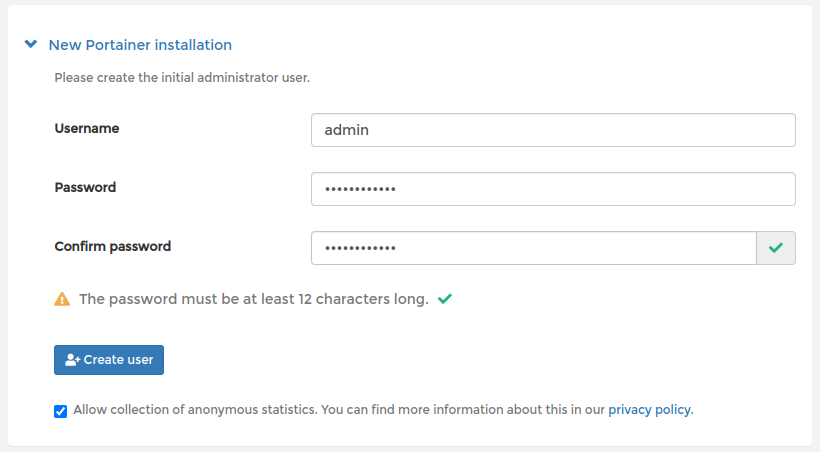
\includegraphics[width=350pt]{chapters/ch-virtualization-and-containerization/figures/portainerlogin.png}
	\caption{Portainer login page to create admin user.} \label{ch:vac:fig:portainerlogin}
\end{figure}

After creating the admin user and logging in, the status of images, containers and many more can be monitored via the dashboard, as shown in Figs. \ref{ch:vac:fig:portainerdashboard1}, \ref{ch:vac:fig:portainerdashboard2} and \ref{ch:vac:fig:portainerdashboard3}. Notice that in Fig. \ref{ch:vac:fig:portainerdashboard3}, using the ``quick action'' buttons, the user can check the specifics of the container and interact with its console, just like using \verb|docker container inspect| and \verb|docker exec|
\begin{figure}
	\centering
	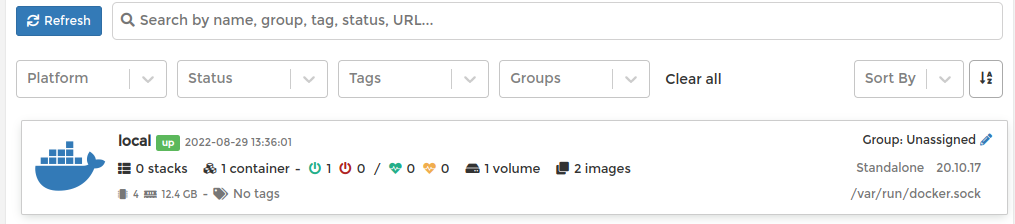
\includegraphics[width=350pt]{chapters/ch-virtualization-and-containerization/figures/portainerdashboard1.png}
	\caption{Portainer dashboard overview of docker servers.} \label{ch:vac:fig:portainerdashboard1}
\end{figure}

\begin{figure}
	\centering
	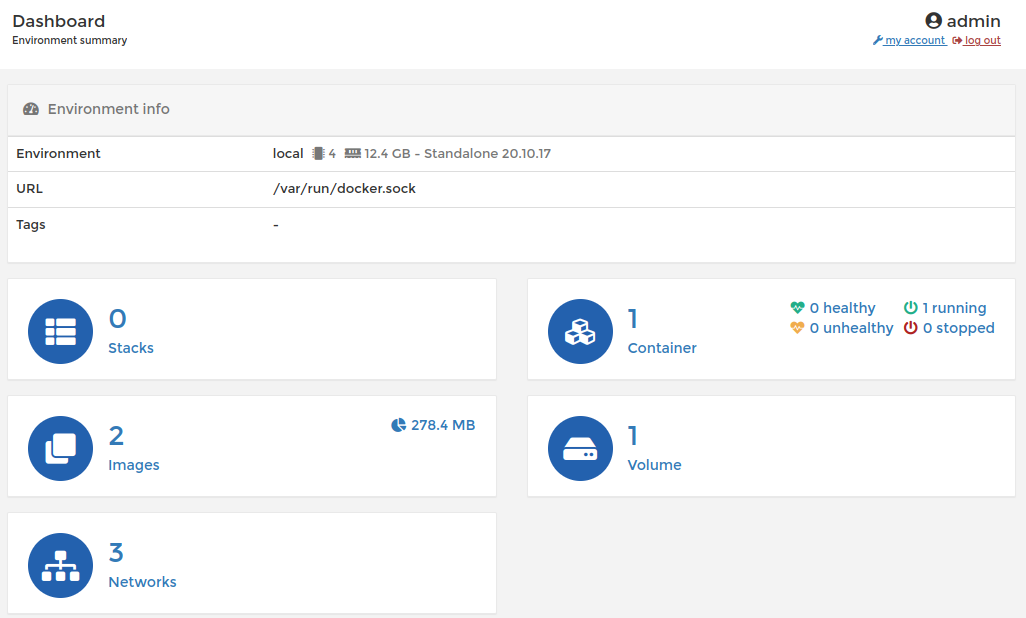
\includegraphics[width=350pt]{chapters/ch-virtualization-and-containerization/figures/portainerdashboard2.png}
	\caption{Portainer dashboard overview in a docker server.} \label{ch:vac:fig:portainerdashboard2}
\end{figure}

\begin{figure}
	\centering
	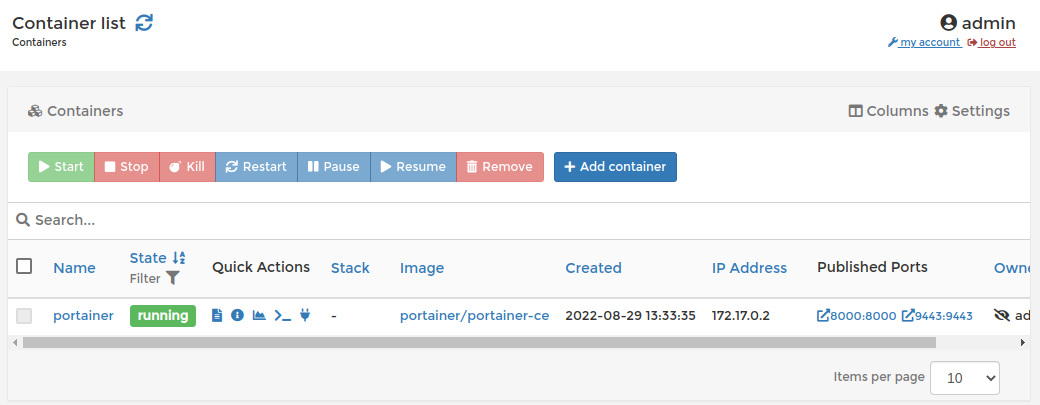
\includegraphics[width=350pt]{chapters/ch-virtualization-and-containerization/figures/portainerdashboard3.png}
	\caption{Portainer dashboard list down of all running containers.} \label{ch:vac:fig:portainerdashboard3}
\end{figure}

In summary, Portainer is an easy-to-use container management tool with clean graphical interface that a user can quickly get used to without a steep learning curve.

\section{Brief Introduction to Kubernetes}

Kubernetes is introduced cross sections. This section focuses on a brief introduction to Kubernetes, its basic schematic architecture, and how it can be installed on a local machine.

\subsection{What is Kubernetes}

\textit{Kubernetes}, also known as \textit{k8s}, is an open-source container orchestration system originally developed by Google. It automates the deployment, scaling, and management of containerized applications. While Kubernetes is more flexible than Portainer, it's also more complex and has a steeper learning curve.

Note that running Kubernetes on a local server can differ significantly from running it on a cloud platform such as AWS or Google Cloud, which offer managed Kubernetes services with additional features and simplified management. These platforms, AWS with its Elastic Kubernetes Service (EKS) and Google Cloud with Google Kubernetes Engine (GKE), have developed their own tools and interfaces for interacting with Kubernetes. So, while learning Kubernetes can be beneficial, one might not need to learn all the low-level details if he is running Kubernetes using one of the above management tools instead of DIY everything.

This notebook focuses introducing running Kubernetes on a local server in a DIY manner. In this scenario, the following common practice is adopted: \textit{kubectl} is used as the user interface to Kubernetes and \textit{minikube} the software to manage the host machine. Minikube is an open-source software developed by the Kubernetes community to run a single-node Kubernetes cluster on a local machine, which is suitable for developers to learn and test different things in development environment.

Notice that in the past days, docker is the default container engine built-in to Kubernetes, and Kubernetes uses a special program ``dockershim'' that talks to docker engine. As of now, docker support is deprecated in Kubernetes and dockershim is removed from the installation.

\subsection{Infrastructure}

Figure \ref{ch:vac:fig:kubernetescluster} demonstrates what key components Kubernetes has inside its cluster.
\begin{figure}
	\centering
	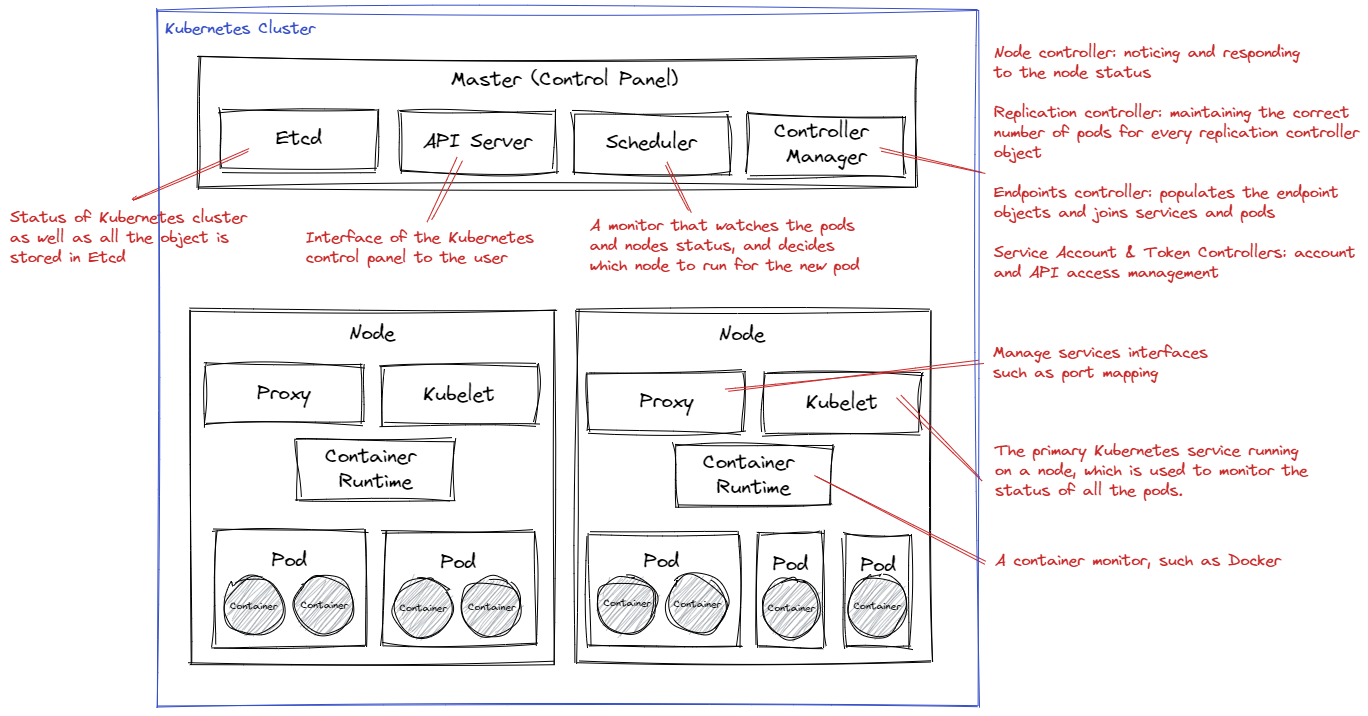
\includegraphics[width=350pt]{chapters/ch-virtualization-and-containerization/figures/kubernetescluster.png}
	\caption{Kubernetes cluster and its key components.} \label{ch:vac:fig:kubernetescluster}
\end{figure}
As shown in Fig. \ref{ch:vac:fig:kubernetescluster}, Kubernetes manages containers in a centralized ``master-worker'' mode, where the master plays as the control panel, API gateway (with static IP address) and load balancer to interact with a user, and the worker nodes (also known as nodes, for short) actually process the data. Each node can host multiple pods, inside each pod is a container or a group of containers that work closely together. Notice that in Kubernetes, containers never run directly in a node. They are always grouped into pods. A pod should be the minimal unit or group of container(s) that can deliver a basic function.

In practice, the master and nodes can run on cross servers or VMs. Kubernetes packages need to be installed on each and every server or VM for the system to work properly. Kubernetes provides variety of tools to distribute the loads to different servers or VMs, or to add redundancy to the system for high availability.

\subsection{Installation}

The installation guidance of Kubernetes can be found at its official website \textit{kubernetes.io}. Notice that different OS adopts different ways of installing and using Kubernetes. The installation procedures introduced in this section applies to Linux OS only. For Windows users, Kubernetes can be installed from Docker desktop. For macOS users, other tools are used to install the tools to be introduced below.

As introduced earlier, \textit{kubectl} is used to interact with Kubernetes. In addition, since we are in development environment, we will also install \textit{minikube} which is used to setup a small Kubernetes cluster in the local machine. They can be installed separately. See following links for more details.
\begin{lstlisting}
https://kubernetes.io/docs/tasks/tools/install-kubectl-linux/
https://minikube.sigs.k8s.io/docs/start/
\end{lstlisting}
When running \textit{minikube} for the first time, it would try to install \textit{kubectl} as a built-in. Start \textit{minikube} using \verb|minikube start|, which will start a VM using Vertual Box, and setup a Kubernetes node in the VM.

If \textit{kubectl} and \textit{minikube} are installed separately, run the following command to verify the successful installation of both software.
\begin{lstlisting}
$ kubectl cluster-info
Kubernetes control plane is running at https://192.168.49.2:8443
CoreDNS is running at https://192.168.49.2:8443/api/v1/namespaces/kube-system/services/kube-dns:dns/proxy
\end{lstlisting}
If \textit{minikube} is installed, and \textit{kubectl} is considered as a built-in installation to \textit{minikube}, use the following command
\begin{lstlisting}
$ minikube kubectl cluster-info
Kubernetes control plane is running at https://192.168.49.2:8443
CoreDNS is running at https://192.168.49.2:8443/api/v1/namespaces/kube-system/services/kube-dns:dns/proxy
\end{lstlisting}
in which case \verb|alias kubectl="minikube kubectl --"| may make things easier.

\section{Basic Kubernetes}

This section focuses on the basic steps of creating a functional Kubernetes cluster.

\subsection{Kubernetes Configuration Files}

Managing containers via container orchestration such as Kubernetes is different from doing so using container engines such as docker engine. Unlike docker engine where we started from building an image from a dockerfile, Kubernetes requires that all images to be used are already available. Instead of having one configuration file where each entry in that file corresponds with a container, when using Kubernetes, multiple configuration files are required, each file corresponding with an object to be created. Notice that an object is not necessarily a container. It can be a pod, a replica controller, a service, or any other ``thing'' in the Kubernetes framework. There are more involving manual setups of networking when using Kubernetes as well. Details are introduced in the remaining of this section.

The following two configuration files are given as examples \cite{stephen2023docker} to demonstrate how these files look like. This example comes from Udemy course \textit{Docker and Kubernetes: The Complete Guide} by Stephen Grinder. They are both written in YAML. Configuration file to setup a pod:
\begin{lstlisting}
apiVersion: v1
kind: Pod
metadata:
    name: client-pod
    labels:
        component: web
spec:
    containers:
        - name: client
          image: <image-name>
          ports:
          	- containerPort: 3000
\end{lstlisting}
Configuration file to setup the networking service:
\begin{lstlisting}
apiVersion: v1
kind: Service
metadata:
    name: client-node-port
spec:
    type: NodePort
    ports:
        - port: 3050
          targetPort: 3000
          nodePort: 31515
    selector:
        component: web
\end{lstlisting}

Commonly used Kubernetes object types are summarized in Table \ref{ch:vac:tab:objtype}.
\begin{table}[htbp]
  \centering
  \caption{Commonly used Kubernetes object types.} \label{ch:vac:tab:objtype}
  \begin{tabularx}{\textwidth}{lX}
    \hline
    Object Type & Description \\
    \hline
    Pod & The smallest and most basic unit in the Kubernetes object model. It represents a single instance of a process running on the cluster. \\ \hdashline
    Deployment & Manages the deployment and scaling of a set of identical pods, ensuring the desired number of replicas are running and providing rolling updates for seamless application upgrades. \\ \hdashline
    Service & Enables network access to a set of pods using a stable IP address and DNS name. It provides load balancing across multiple pod replicas and allows external traffic to be directed to the appropriate pods. \\ \hdashline
    ConfigMap & Stores configuration data in key-value pairs, which can be consumed by pods as environment variables, command-line arguments, or mounted as files. \\ \hdashline
    Secret & Similar to a ConfigMap, but specifically designed to store sensitive data, such as passwords, API keys, and TLS certificates. Secrets are encrypted at rest and can be mounted into pods as files or exposed as environment variables. \\ \hdashline
    PersistentVolume & Provides a way to provision and manage persistent storage resources in a cluster. It decouples the storage from the underlying infrastructure and allows data to persist beyond the lifecycle of individual pods. \\ \hdashline
    PersistentVolumeClaim & Requests a specific amount of storage from a PersistentVolume. It acts as a request for a specific storage resource and provides an abstraction layer for managing persistent storage in a cluster. \\ \hdashline
    Ingress & Manages external access to services within a cluster. It acts as a reverse proxy and exposes HTTP and HTTPS routes to route traffic to the appropriate services based on hostnames, paths, or other rules. \\
    \hline
  \end{tabularx}
\end{table}
Some highlights of the above configuration files are as follows.
\begin{itemize}
  \item \verb|apiVersion| plays as the prefix that decides what configuration types are supported. For example, under the scope of \verb|v1|, \verb|Pod|, \verb|Service|, \verb|configMap|, \verb|Namespace|, etc., are supported. In a different \verb|apps/v1|, a different set of configuration types \verb|ControllerRevision|, \verb|StatefulSet|, etc., are supported. It's important to choose the correct apiVersion for the Kubernetes API version you are working with to ensure the compatibility and availability of the desired configuration options.
  \item \verb|kind| This indicates the type of the object that the configuration file describes. For example, \verb|Pod| represents a pod that is used to host containers, and \verb|Service| the primary object type that defines networking, with subtypes \verb|NodePort| (see example above), \verb|ClusterIP|, \verb|LoadBalancer| and \verb|Ingress|.
  \item \verb|metadata| indicates the name and labels of the object. For example, \verb|component: web| is defined as a label of the pod. This information is passed to the networking service under \verb|selector|, so that the networking service knows which object it should link to.
  \item \verb|port|, \verb|targetPort| and \verb|nodePort| are used to specify ports used in the service. The \verb|targetPort| indicates which port in the pod should be exposed to the service, and it is consistent with \verb|containerPort| defined in the pod. Assume that there is another pod in the node who needs to talk to this pod via the service. The other pod's port that communicates with the service is fed into \verb|port|. Finally, \verb|nodePort| is the port with value between 30000 and 32767 that is exposed from the service to outside the node. If \verb|nodePort| is not assigned, a random number within the range will be assigned. This is shown in Fig. \ref{ch:vac:fig:nodeport}.
\end{itemize}
Notice that Kubernetes networking using \verb|kind: Service| is more complicated than shown in the above example. More details of it is given later in a dedicated Section \ref{ch:vac:subsec:k8snetworking}.

\begin{figure}
	\centering
	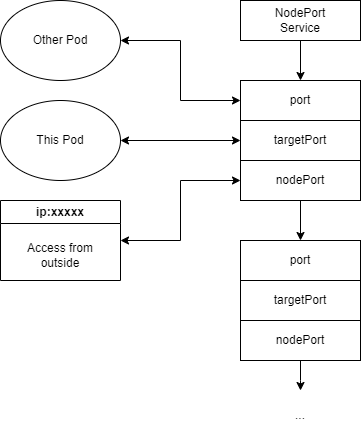
\includegraphics[width=200pt]{chapters/ch-virtualization-and-containerization/figures/nodeport.png}
	\caption{The NodePort networking service.} \label{ch:vac:fig:nodeport}
\end{figure}

\subsection{Cluster Deployment}

With the image and the configuration files ready, the next step is to deploy the nodes, pods, and containers. \textit{kubectl} command line interface is used to instruct Kubernetes to deploy the objects as follows.
\begin{lstlisting}
$ kubectl apply -f <configuration file>
\end{lstlisting}
This essentially asks the master node in the Kubernetes cluster to start taking actions according to the configuration files, such as to inform the nodes to start creating pods and containers. The master node also keeps monitoring the status of each work node, to make sure that everything is running as planned. If there is a container failure, etc., the master node will guide the associated note to restart the container.

It is worth mentioning here that by default Kubernetes uses declarative deployment instead of imperative deployment, meaning that the developer does not need to specifically tell Kubernetes what to do in each step. The developer only tells the overall objectives, and Kubernetes master node will try to figure out the steps to realize that goal. It is possible to enforce Kubernetes master node to practice specific details via configuration files, but it is almost always recommended to use the default declarative approach with Kubernetes.

To retrieve information, such as the status, of a group of objects, use
\begin{lstlisting}
$ kubectl get <object type>
\end{lstlisting}
where \verb|<object type>| can be \verb|pods|, \verb|services|, etc. For more details of a specific object, use
\begin{lstlisting}
$ kubectl describe <object type> <object name>
\end{lstlisting}
for example, to check the containers running in a pod. If \verb|<object name>| is neglected, Kubernetes returns detailed information of all objects of the given object type. For a running object, use
\begin{lstlisting}
$ kubectl logs <object name>
\end{lstlisting}
to check the log file of that object.

With the above been done, open a browser and use \verb|<ip>:<port>| to access the application running in the container, where \verb|<ip>| is the IP address of the VM (not \verb|localhost|) that \textit{minikube} created, and \verb|<port>| the port configured in NodePort service under \verb|nodePort|. The IP address can be found by running \verb|minikube ip|.

\subsection{ClusterUpdate} \label{ch:vac:subsec:updatek8s}

Without container orchestration such as Kubernetes, one of the most challenging tasks is to update the container for a different configuration, for example, changing the underlying image. With the help of Kubernetes declarative approach, it is possible update the cluster simply by revising the configuration files, and pass them to Kubernetes as if the cluster is to be deployed for the first time. Kubernetes automatically checks the names and kinds of the revised configuration files, comparing them with existing running objects, and update them if necessary.

Check the status of the pods using \verb|kubectl get pods|. After updating, the pods are often restarted, hence it is expected to see increment in the ``RESTARTS'' tag. To double confirm that updates have been made, use \verb|kubectl describe| to check the details of the relevant objects.

However, there is a limitation to the updating of the Kubernetes deployment. For an existing object, only certain fields in the configuration files can be changed. For example, for a pod that runs containers, the image can be changed, but the container port cannot. Sometimes there can be a walk around. For example, in the case of changing container port of pods, consider using a new object type \verb|Deployment| instead of \verb|Pod|, which allows more flexible updating. The \verb|Deployment| in its backend is consist of one or more monitored and managed identical pods.

To revert \verb|kubectl apply|, i.e., to remove a configuration file, use
\begin{lstlisting}
$ kubectl delete -f <configuration file>
\end{lstlisting}
Kubernetes treats the above delete command as a specific type of update to the cluster, and will action accordingly.

\section{Advanced Kubernetes}

This section introduces advanced commonly used Kubernetes objects, tools and techniques.

\subsection{Kubernetes Object: Deployment} \label{ch:vac:subsec:deployment}

As introduced in Section \ref{ch:vac:subsec:updatek8s}, updating pods has some limitations. It is practically more convenient to setup pods using ``Deployment'' object instead of ``pod''. The Deployment object servers as an additional layer of Kubernetes infrastructure that manages identical pods. More details of Deployment object is introduced in this section.

As an example, here is a configuration file from Kubernetes manual that deploys a Deployment object.
\begin{lstlisting}
apiVersion: apps/v1
kind: Deployment
metadata:
  name: nginx-deployment
  labels:
    app: nginx
spec:
  replicas: 3
  selector:
    matchLabels:
      app: nginx
  template:
    metadata:
      labels:
        app: nginx
    spec:
      containers:
      - name: nginx
        image: nginx
        ports:
        - containerPort: 80
\end{lstlisting}
Some highlights are as follows.
\begin{itemize}
  \item \verb|replicas| gives the expected number of pods that the Deployment object manages.
  \item \verb|matchLabels| specifies the pods with which label are to be managed by the Deployment object. In this example, the label is \verb|app: nginx|. When populating pods, the pods would have the same label, as the same label is assigned under \verb|template|, \verb|metadata|, \verb|labels|.
  \item \verb|template| specifies the template that is used to create the pods.
\end{itemize}

When a new version of an image becomes available, we may want to update the containers accordingly. Re-apply the same configuration file would not help, as Kubernetes would reject apply request if no change is detected in the configuration file. It would not check whether the image is in its latest version. Kubernetes uses the following imperial command to update images as a walk around, and the developer needs to run this command manually.
\begin{lstlisting}
$ kubectl set image deployment/<Deployment name> <container name>=<image name>
\end{lstlisting}
For example,
\begin{lstlisting}
$ kubectl set image deployment/nginx-deployment nginx=nginx:1.25.1
\end{lstlisting}

\subsection{Kubernetes Object: Service} \label{ch:vac:subsec:k8snetworking}

There are 4 service types defined in Kubernetes. So far ``NodePort'' service type has been introduced in earlier examples. More types are introduced here.

A summary of different service types are given below.
\begin{itemize}
	\item ClusterIP: Exposes the service object on a cluster-internal IP. Objects in the cluster can access to the object that a ClusterIP is pointing at.
	\item NodePort: Assigns a static port with the cluster IP, and exposes the service object to the internet. This is used mostly used in development environment, not in production environment.
	\item LoadBalancer: Exposes the service object externally using an external load balancer. Kubernetes does not provide built-in load balancer.
	\item ExternalName: Maps the service object to the contents of the \verb|externalName| field, such as a host name. This is related to cluster DNS server.
\end{itemize}

A ClusterIP configuration file may look like the following.
\begin{lstlisting}
apiVersion: v1
kind: Service
metadata:
	name: client-cluster-ip-service
spec:
	type: ClusterIP
	selector:
		<target tag>
	ports:
		- port: <port for internal comm>
		  targetPort: <port for internal comm>
\end{lstlisting}
where the first \verb|port for internal comm| is the port in the ClusterIP service object that opens to other objects in the cluster, and the second the port the target object opens to the ClusterIP service object. They can be set differently, but usually they are just set to the same value.

\subsection{Kubernetes Object: Persistent Volume Claim, Persistent Volume, and Volume} \label{ch:vac:subsec:k8svolume}

Docker engine uses volumes to maintain persistent data and share data among containers. Details have been introduced in Section \ref{ch:vac:subsec:dockervolume}. Kubernetes volume framework is similar in the sense that it makes sure that the data is saved and managed by the host machine, so that when the pods or containers are shutdown or restarted, the data can be restored safely.

Do notice that when comes to data sharing using volume, it is dangerous to have multiple containers or the host machine accessing the same files simultaneously, without knowing the existence of each other. Usually additional steps need to be setup to ensure data consistency.

It is worth emphasizing the differences of ``volume'' technology in containerization and Kubernetes volume-related objects: Persistent Volume Claim (PVC). Persistent Volume (PV), and Volume. As a matter of fact, Kubernetes Volume object is usually not what we want. Kubernetes Volume creates the volume tied to a pod, not to the host machine. It survives container failure in the pod, but not pod failure. In summary:
\begin{itemize}
	\item Kubernetes Volume: A volume tied to the pod. It survives container failure inside the pod, but not pod failure.
	\item Kubernetes PV: A volume tied to the host machine. It survives pod failure. It can be provisioned either automatically by a StorageClass, or manually by the developer and administrator.
	\item Kubernetes PVC: It is essentially a request sent from a pod or a container, asking for specific amount of storage from a PV. Kubernetes will find that amount of PV from either existing provisioned static PV, or dynamically provision new ones for the pod or container.
\end{itemize}
A Deployment or a pod can claim a PV using a PVC, in which case a PV will be provisioned following the PVC requirements. There is a one-to-one relationship between the PV and the PVC. If there are multiple pods, each requiring a dedicated PV, then multiple PVCs must be used. The developer can either create those PVCs manually, or use a Volume Claim Template to claim them if they are similar.

An example of claiming Kubernetes PV and PVC is given below. In the remaining part of this section, we will be mostly using PVC instead of PV.
\begin{lstlisting}
# persistent-volume.yaml

apiVersion: v1
kind: PersistentVolume
metadata:
	name: my-pv
spec:
	storageClassName: standard
	capacity:
		storage: 10Gi
	accessModes:
		- ReadWriteOnce
	hostPath:
		path: /data/my-pv
---
# persistent-volume-claim.yaml

apiVersion: v1
kind: PersistentVolumeClaim
metadata:
	name: my-pvc
spec:
	storageClassName: standard
	accessModes:
		- ReadWriteOnce
	resources:
		requests:
			storage: 5Gi
\end{lstlisting}
To check the PV objects, use \verb|$ kubectl get pv| and \verb|$ kubectl get pvc|.

To add the above Kubernetes PVC to a Kubernetes Deployment, add volumes information to the specs as given in the following example.
\begin{lstlisting}
apiVersion: apps/v1
kind: Deployment
metadata:
	name: my-app-deployment
spec:
	replicas: 1
	selector:
		matchLabels:
			app: my-app
	template:
		metadata:
			labels:
				app: my-app
		spec:
			containers:
				- name: my-app-container
				  image: my-app-image
				  ports:
					- containerPort: 8080
				  volumeMounts:
					- name: data-volume
					  mountPath: /data
					  subPath: data-from-container
			volumes:
				- name: data-volume
				  persistentVolumeClaim:
					claimName: my-pvc
\end{lstlisting}
where \verb|volumes| defines which Kubernetes PVC is used, and \verb|volumeMounts| tells how it is mounted in the container. The \verb|mountPath| is the path in the container whose data is mounted by the volume. If a \verb|subPath| is given, a sub-folder of its specified name will be created in the host machine in the volume to contain the data.

There are different types of access modes: 
\begin{itemize}
\item \verb|ReadWriteOnce|: Allow one node to read and write at a time.
\item \verb|ReadOnlyMany|: Allow many nodes to read at a time.
\item \verb|ReadWriteMany|: Allow many nodes to read and write at a time.
\end{itemize}

It is worth mentioning that it can be controlled where Kubernetes would look for storage by default. On a personal PC, this would of course most likely to be the hard drive, or a virtual storage space in the VM. Use the following command to check Kubernetes possible choice of storage.
\begin{lstlisting}
$ kubectl get storageclass
\end{lstlisting}
and 
\begin{lstlisting}
$ kubectl describe storageclass
\end{lstlisting}
However, when deploying Kubernetes on a Cloud provider, the developer needs to configure where to slice the PV, as there would be many storage options. Usually, each Cloud provider will have its own default storage space for Kubernetes, such as AWS Elastic Block Store for AWS.





\subsection{Kubernetes Multi-Container Application}

In this section, we are using an example to demonstrate the general workflow of a multi-container application deployment using Kubernetes. The example is from \cite{stephen2023docker}.

A general framework of the deployment is given in Fig. \ref{ch:vac:fig:multipodk8s}. It would be too detailed to explain how each part of the deployment functions. Only some highlights are introduced.
\begin{figure}
	\centering
	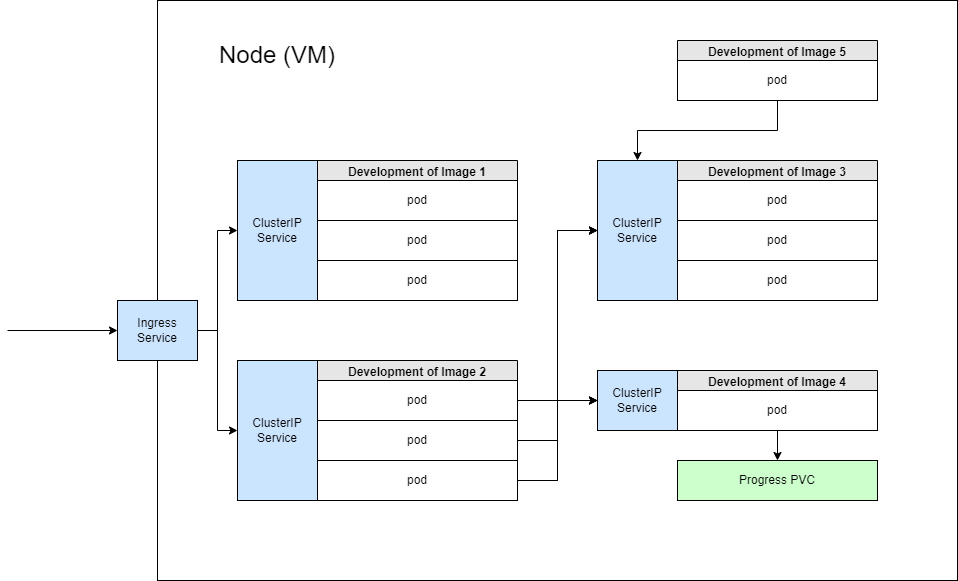
\includegraphics[width=350pt]{chapters/ch-virtualization-and-containerization/figures/multipodk8s.png}
	\caption{A multi-container deployment example given in \cite{stephen2023docker}.} \label{ch:vac:fig:multipodk8s}
\end{figure}

The developer needs to prepare at least 11 configuration files for this implementation, each associated with a colored object in  Fig. \ref{ch:vac:fig:multipodk8s}. The blocks in blue are associated with communication-relevant objects, gray pods-relevant objects, and green the volume claim.

The configuration files for deploying pods using Deployment object and constructing internal communications using ClusterIP service object have already been introduced in Section \ref{ch:vac:subsec:deployment} and \ref{ch:vac:subsec:k8snetworking}, respectively. 

To apply a group of configuration files all together, provide the directory name of all the configuration files to Kubernetes instead of feeding each configuration file one at a time.
\begin{lstlisting}
$ kubectl apply -f <directory>
\end{lstlisting}
When directory is given instead of a file, Kubernetes will try to apply all the configuration files in that directory.

It is possible to consolidate the configuration files of objects into one conjunctive configuration file. To do that, use \verb|---| to split the configurations for each object in the conjunctive configuration file as follows. It is of personal preference whether to use conjunctive configuration files or separate configuration files for all objects.
\begin{lstlisting}
<configurations-for-object-1>
---
<configurations-for-object-2>
---
<...>
\end{lstlisting}













\section{Docker Hub}

Docker Hub is a commonly used server for storing and sharing docker images. It is also the default remote repository server of Docker engine. However, do notice that Docker Hub is not the only remote docker image server. Some alternatives are Amazon Elastic Container Registry, Red hat Quay, Azure Container Registry, Google Container Registry, etc.

After registering an account on Docker Hub, use the following command to login to the docker hub from your local machine.
\begin{lstlisting}
$ docker login --username=<user name>
Passowrd:
\end{lstlisting}

Assume that there is an image in the local machine, and an empty repository on Docker Hub. In order to push the local image to the Docker Hub, the first step is to add the remote repository and the ``\textit{RepoTags}'' in the local image as follows.
\begin{lstlisting}
$ docker tag <image name> <username>/<repository name>:<version>
\end{lstlisting}
where \verb|<version>| is a tag usually used to distinguish the different branches or versions of the images on Docker Hub. For the first image upload, it can simply be \verb|latest|.

Use the following command to push the image to Docker Hub.
\begin{lstlisting}
$ docker push <user name>/<repository name>
\end{lstlisting}




